\documentclass[dvipdfmx]{jarticle}
\usepackage{tikz}
\pagestyle{empty}
\usetikzlibrary{shapes,calc}
\begin{document}
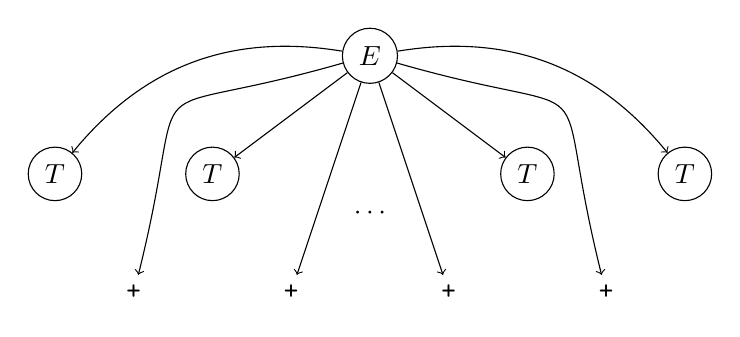
\begin{tikzpicture}
  \node[circle,draw] (N0) at (0,0) {$E$};
  \node (N1) at (-3,-3) {$\texttt{+}$};
  \node[circle,draw] (N2) at (-4,-1.5) {$T$};
  \node (N3) at (-1,-3) {$\texttt{+}$};
  \node[circle,draw] (N4) at (-2,-1.5) {$T$};
  \node at (0,-2) {$\cdots$};
  \node (N5) at (1,-3) {$\texttt{+}$};
  \node[circle,draw] (N6) at (2,-1.5) {$T$};
  \node (N7) at (3,-3) {$\texttt{+}$};
  \node[circle,draw] (N8) at (4,-1.5) {$T$};

  \path[->] (N0) edge[bend right] (N2) (N0) edge [bend right,looseness=2] (N1)
            (N0) edge (N3) (N0) edge (N4);
  \path[->] (N0) edge (N5) (N0) edge (N6)
            (N0) edge [bend left,looseness=2] (N7) (N0) edge [bend left] (N8);
\end{tikzpicture}
\end{document}